\chapter[Implementácia]{Implementácia softvéru}
\label{kap:implementacia}

V tejto kapitole uvedieme, ako sme postupovali pri implementácií softvéru. Odhalíme, aké postupy, štruktúry či algoritmy sme zvolili, pričom popíšeme aj dôvody nášho výberu. Neuvádzame celý kód, ale len tie časti, ktoré sa nám zdali byť najviac zaujímavé a zodpovedajúce obsahu našej práce.\newline


\section{Prvé myšlienky}

V prvom rade je zo všetkého najdôležitejšie ujasniť si, aké ciele má spĺňať naša implementácia. Treba si uvedomiť, čo chceme, aby náš program vedel robiť, jemne si načrtnúť, ako potrebné veci naprogramovať, ale tiež v akom poradí na nich pracovať.\newline

Prvoradý a najpodstatnejší cieľ našej práce je dozaista vyhľadávač spojení v grafikone mestskej hromadnej dopravy. Teraz rozoberieme, čo všetko jeho implementácia obnáša.\newline

Na začiatok budeme potrebovať vytvoriť, prípadne získať dáta, s ktorými budeme pracovať. Tie môžeme buď náhodne vygenerovať, pre vlastnú potrebu a testovanie aplikácie prevziať dáta z už existujúcej siete MHD, alebo si vytvoriť nejaké vlastné, sofistikované testovacie vstupy. Každá možnosť má svoje kladné i záporné stránky. Náhodné dáta otestujú algoritmy veľmi slušne, avšak môžu obsahovať rôzne anomálie a pravdepodobne ani zďaleka nebudú zobrazovať reálny tvar grafikonu MHD. Prevzaté dáta z existujúcich MHD tieto nedostatky znamenite riešia. Ich nevýhodou je ale ich použitie len na lokálne účely, nakoľko nemôžu byť publikované verejne. Vlastne vytvorené vstupy sú zasa výborné na testovanie okrajových prípadov, na nachádzanie a odstraňovanie chýb v programe, ako i na skúšanie programu pri malých zmenách v algoritme a pozorovaní očakávaných výsledkov. Naopak ale, postrádajú prítomnosť rozmerných dátových súborov, keďže ručné vytváranie objemných dát je časovo priveľmi náročné.\newline

V našich mysliach teda leží otázka, aké dáta zvoliť ako vstup. Samozrejme najlepšie by bolo použiť všetky tri spomínané možnosti. My sa však uspokojíme iba s dvomi z nich. Pri vytváraní kódu bude veľmi vhodné využívať nami navrhnuté vstupy, ktoré otestujú práve vytváranú časť programu. Po vytvorení zdanlivo funkčnej aplikácie ju otestujeme na existujúcich dátach, pričom zistíme či je program dostatočne rýchly a či sú jeho výstupy uspokojivé v porovnaní s inými vyhľadávačmi spojení. Náhodne generované vstupy nebudeme používať, keďže pomocou kombinácie predošlých dvoch zistíme všetky potrebné informácie o funkčnosti aplikácie.\newline

Treba si tiež premyslieť, kde si budeme spomínané dáta uschovávať. Za uváženie stoja dve možnosti. Dáta držať v textovom súbore alebo ich načítať do nejakej databázy, a z nej potom čerpať. Textová reprezentácia je všestranná, ľahko s ňou pracovať i meniť vstupné údaje. Jej načítanie môže ale spomaľovať chod našej aplikácie. Naproti tomu, databáza je rýchla na čítanie z nej, ale jej o niečo ťažšie vytváranie znepríjemňuje našu snahu o testovanie mnohých vlastných vstupov. My sme, nakoľko je to jednoduchšie, zvolili textovú reprezentáciu dát. Opäť, najvhodnejšie by bolo oba spôsoby skombinovať, a teda uschovávať údaje v textových súboroch a nejaký vybraný vstup mať uložený v databáze.\newline

Ďalším bodom, o ktorom radno pouvažovať, je reprezentácia týchto údajov. Pre začiatok volíme znova čo najjednoduchšiu možnosť: vrcholmi nami používaného grafu budú zastávky MHD a hranami sa stanú linky jazdiace medzi nimi. Tu, keďže sme si vybrali takú jednoduchú alternatívu, nesmieme zabúdať na flexibilitu. Ak sa ukáže nejaký problém, netreba sa báť reprezentáciu údajov rozumne pozmeniť, aby sme si zbytočne nenarobili problémy, ktoré sa budú v neskorších častiach implementácie náročne odstraňovať.\newline

Nasledujúcou zastávkou je vytvorenie objektov na reprezentáciu grafu. Už sme spomínali, že budeme pracovať s orientovanými grafmi. Sprvu si vystačíme s hodnotením hrán. Teraz presnejšie popíšeme objekty, ktoré si budú držať informácie o vrcholoch, hranách i o celom grafe a budú tak reprezentovať uvedené grafové štruktúry. Riešenie je nateraz triviálne: Trieda vrcholu moc informácií nepotrebuje. Nech je jej premennou len názov zastávky. Trieda hrany bude vyžadovať referencie na dva vrcholy, keďže sme tak hrany v kapitole \ref{kap:grafy} definovali, a premennú predstavujúcu hodnotiacu funkciu. Táto implementácia sa jemne líši od našej definície hodnotiacej funkcie, avšak uvedeným spôsobom poľahky dosiahneme všetky predpoklady spomínanej funkcie. Ak poznáme hranu, v konštantnom čase vieme zistiť jej hodnotenie, keďže len pristúpime k zodpovedajúcej premennej. Nakoniec, trieda grafu bude obsahovať dve polia reprezentujúce všetky hrany a všetky vrcholy v grafe.\newline

V tejto chvíli je prvotne premyslená celá reprezentácia údajov a prichádza na rad výber vyhľadávacieho algoritmu. Rozdiely medzi uvedenými algoritmami sa nachádzajú na konci predošlej kapitoly (\ref{vyhlad_alg_zhrnutie}). Z nich vychádzajúc sme usúdili, že najvhodnejšie bude implementovať Dijkstrov algoritmus. Naše úvahy vychádzali prevažne z nami vytýčených cieľov, a teda funkcionality programu na reálnych dátach, ktoré sú vo väčšine prípadov veľké zoskupenia údajov. Z tohto dôvodu je nevhodný ako Bellman\textendash Fordov, tak i Floyd\textendash Warshallov algoritmus. Dijkstra navyše spoľahlivo a rýchlo funguje aj na menších vstupoch a pre jeho všestrannosť je najlepším kandidátom pre riešenie našich cieľov.\newline

V našom hypotetickom modeli už teda dokážeme zistiť výsledok vyhľadávania. Avšak musíme ešte ošetriť, kam sa želaný stav uloží, aby bolo jednoduché ho vypísať. A taktiež si treba rozmyslieť, ako chceme výsledky vypisovať. Ako sme už spomínali v kapitole \ref{kap:algoritmy}, budeme používať implementáciu vyhľadávacieho algoritmu s pamätaním si predchádzajúcich vrcholov pre nájdené najlacnejšie cesty, aby sme boli schopný ich zrekonštruovať. Mohli by sme teda vytvoriť nové pole o veľkosti počtu vrcholov grafu, do ktorého si tieto referencie uložíme. My však použijeme rovnaký postup ako pri hodnotiacej funkcií, a teda do objektu vrchola pridáme premennú držiacu si referenciu na predchádzajúci vrchol. Toto riešenie ale nie je najšťastnejšie, keďže objekt vrchola nemá čo do činenia s výsledkom vyhľadávania najlacnejších ciest v grafe. Správne by bolo všetky vrcholy obaliť ďalším objektom s príznačným názvom a v ňom si držať túto informáciu. V našom prípade ale ide o celkovo nie až tak ťažký kód, preto je takéto jemné zneprehľadnenie akceptovateľné. Vďaka memorizácií predchodcu vrchola nám teda stačí pri výpise poznať cieľovú zastávku vyhľadávania a dokážeme poľahky vyhotoviť žiadanú cestu. Pre začiatok sa uspokojíme s výpisom do konzoly, čo nám postačí až do záverečných prác na aplikácií.\newline

Zostávajúcemu cieľu, čo je implementácia vylepšenia, sme sa rozhodli venovať a premýšľať nad ním až po uskutočnení doteraz opisovaného cieľa.\newline

Po prejdení si všetkých potrebných úvah nám ale stále zostáva jedna nezodpovedaná otázka. Musíme si vybrať programovací jazyk, prípadne prostredie, v ktorom naše myšlienky zrealizujeme. Znalosť potrebných vecí na implementáciu nám ale výrazne pomôže pri našom výbere. Nakoľko budeme chcieť reprezentovať graf, jeho vrcholy i hrany, bude nanajvýš priaznivé zvoliť objektovo orientovaný jazyk. Na myseľ prichádza Java, C\#, Python, JavaScript. Ďalším kritériom je, že v aplikácií budeme od používateľa požadovať vstupné parametre v podobe počiatočnej a koncovej zastávky. Budeme teda vytvárať nejaké okná, textové polia a tlačidlá. Tieto možnosti sú už predpripravené, spolu s mnohými inými, vo vývojom prostredí Unity. Ide o prostredie určené prevažne na vývoj počítačových hier, avšak pre naše účely je úplne dokonalé. Využijeme jeho možnosť programovania v jazyku C\# a hojne i jeho grafické rozhranie.\newline


\section{Začiatočná implementácia}

Po dôkladnom premyslení si všetkých potrebných detailov sme prešli k prvej implementácií. Samozrejme, nevyriešili sme ich všetky. Hneď, ako sme chceli vytvoriť prvý testový vstup, zistili sme, že sme si neujasnili, v akom formáte budeme dáta uschovávať. Ich formát je nepodstatný pre beh aplikácie, keďže si dáta v programe ihneď spracujeme na nami navrhnuté štruktúry. Stačí teda zvoliť ľubovoľný rozumný. Náš je demonštrovaný na obrázku \ref{Format_datoveho_suboru}.\newline

\begin{figure}[H]
  \centering{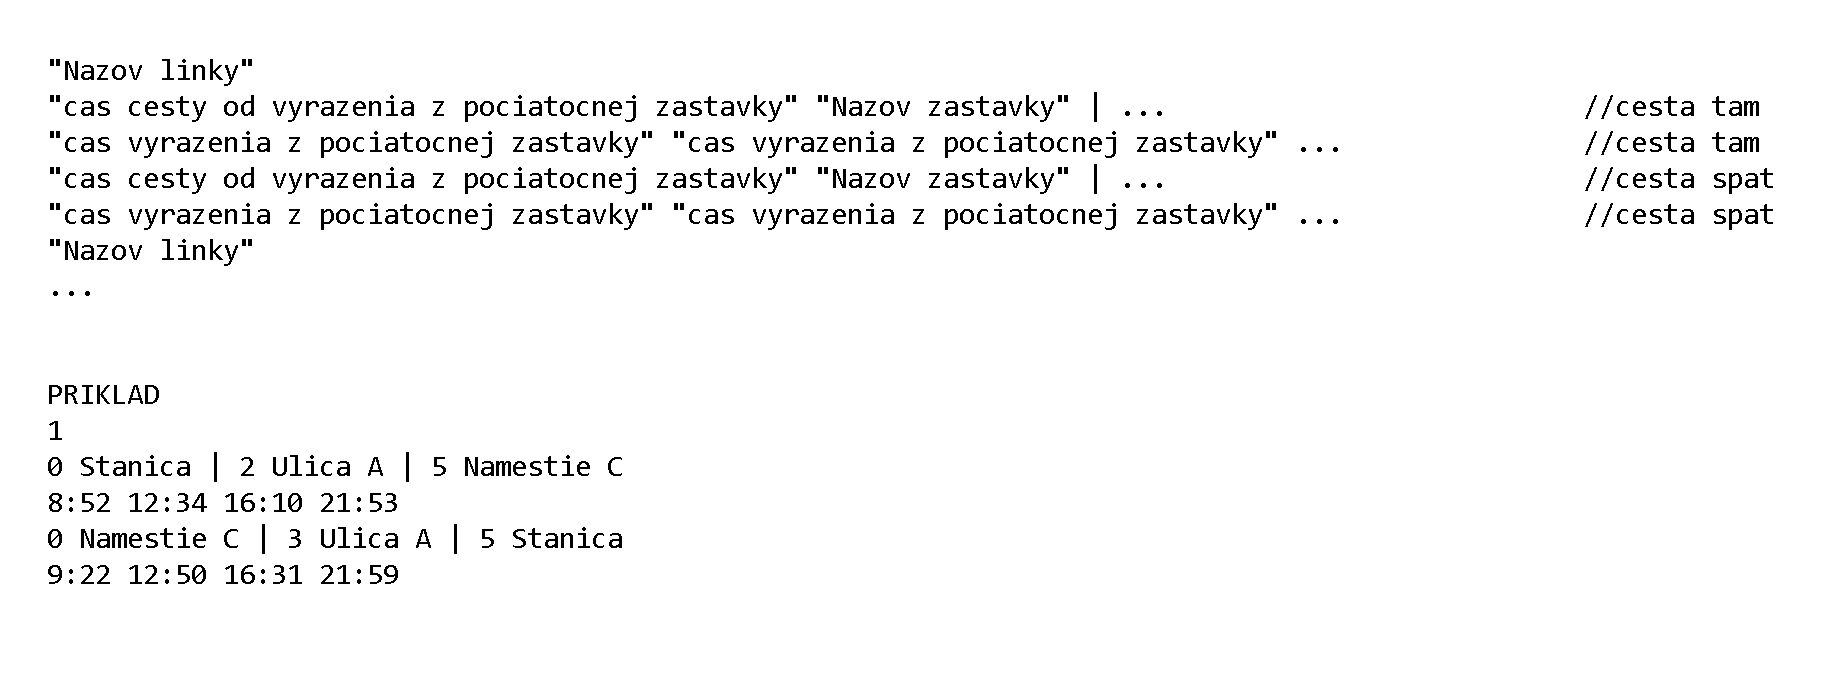
\includegraphics[width=\linewidth]{./images/Format_datoveho_suboru.png}}
  \caption{Formát obsahu dátového súboru}
  \label{Format_datoveho_suboru}
\end{figure}

Teraz môžeme smelo zbierať dáta. Vďaka stránke Bratislavského dopravného podniku sme si uložili dáta popisujúce mestskú hromadnú dopravu v Bratislave. Tie použijeme lokálne na testovanie aplikácie. Vytvorili sme aj pár vlastných vstupov. Na obrázku \ref{priklad_vstupu_1} uvádzame ich jednoduchý príklad. V ňom sme uvažovali o linke vyrážajúcej z A do C v časoch 0:2 a 0:5 so spiatočnou cestou iba z C do B v čase 0:1.\newline

\begin{figure}[H]
  \centering{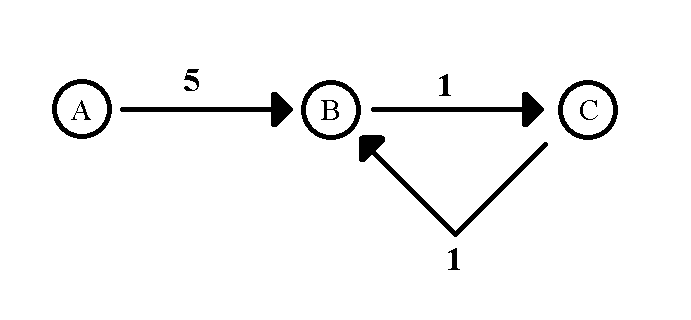
\includegraphics[width=\linewidth]{./images/test2_priklad1.png}}
  \caption{Príklad testového vstupu}
  \label{priklad_vstupu_1}
\end{figure}

Nasleduje implementácia grafových štruktúr, ktorá je nateraz jednoduchá. Vhodné je poznamenať, že v našej implementácií vrchola, ktorú zachytáva obrázok \ref{1_Vertex} , si budeme pamätať hodnotu najlacnejšej cesty do daného vrcholu, aby sme v Dijkstrovom algoritme nepotrebovali vytvárať pole čísel uchovávajúce jeho výsledky. Taktiež si budeme pamätať i referenciu na hranu, ktorá tento vrchol spája s jeho predchodcom, čo nám uľahčí budúcu prácu.\newline

\begin{figure}[H]
  \centering{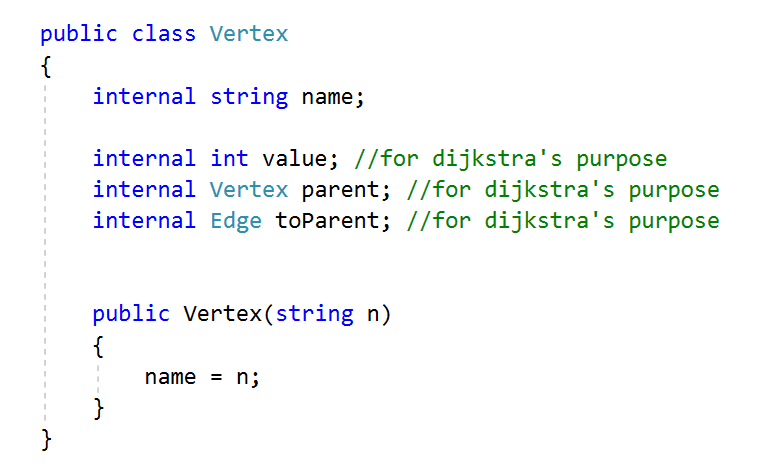
\includegraphics[width=0.7\linewidth]{./images/1_Vertex.png}}
  \caption{Prvá reprezentácia vrcholu}
  \label{1_Vertex}
\end{figure}

Kód pre objekt hrany má ešte navyše pridané časy príchodu a odchodu linky z daných vrcholov. Inak objekty reprezentujúce hranu a graf neobsahujú žiadne zmeny.\newline

\begin{figure}[H]
  \centering{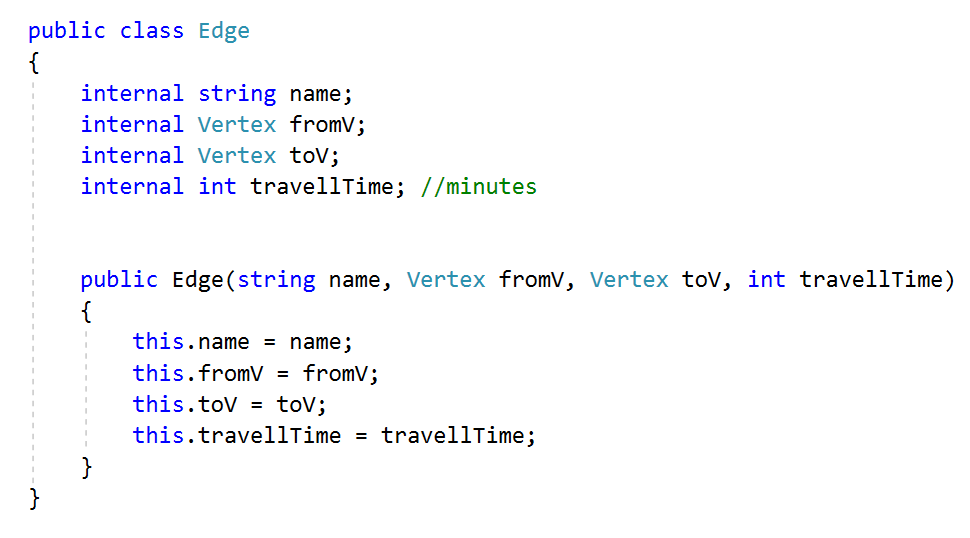
\includegraphics[width=0.7\linewidth]{./images/1_Edge.png}}
  \caption{Prvá reprezentácia hrany}
  \label{1_Edge}
\end{figure}

\begin{figure}[H]
  \centering{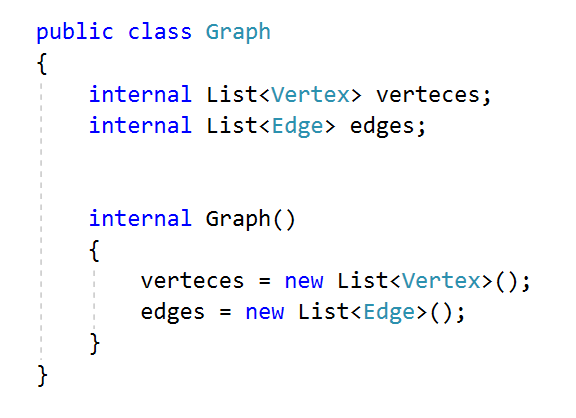
\includegraphics[width=0.7\linewidth]{./images/1_Graph.png}}
  \caption{Prvá reprezentácia grafu}
  \label{1_Graph}
\end{figure}

Pri vytváraní kódu bolo tiež potrebné rozobrať súbor s dátami a vytvoriť z nich horeuvedené objekty. Tento kód uvádzať nebudeme, nakoľko je dosť obsiahly a navyše neobsahuje žiadne relevantné informácie.\newline

Ďalším krokom je implementácia vyhľadávacieho algoritmu. Tu však badáme komplikáciu. Medzi dvomi vrcholmi/zastávkami sa nachádza mnoho hrán reprezentujúcich všetky spojenia medzi nimi. Treba pomocou algoritmu zistiť, ktorú z týchto hrán vybrať. Najlepšie by bolo nejako vyberať hrany čo najskôr po udanom čase, od ktorého chceme vyhľadávať. To by však potrebovalo premnoho modifikácií algoritmu. My sme sa preto rozhodli riešiť tento problém zmenou reprezentácie údajov.\newline


\section{Vylepšenie reprezentácie údajov}

Keďže nám predošlá reprezentácia údajov spôsobovala komplikácie pri vyhľadávaní, rozhodli sme sa ju prerobiť. Nejde o priveľmi signifikantnú zmenu, avšak jej dopad na vyhľadávanie bude nanajvýš uspokojujúci. Zmenou je, že naše vrcholy nebudú reprezentovať len zastávku, ale aj čas, v ktorom sa niečo v tej zastávke deje. Napríklad pre linku idúcu zo zastávky $A$ do $B$ v čase 0:1 s príchodom 0:6 vytvoríme dva vrcholy, jeden s hodnotami $A$ a 0:1 a druhý s údajmi $B$ a 0:6, pričom uvažovaná hrana spája presne tieto dva vrcholy. Tým pádom budeme nútení vytvoriť veľa hrán navyše, a to hrany, na ktorých sa čaká na nejakej zástavke. My sme tieto hrany nazvali "čakacie". Napríklad ak by bol v poslednom príklade práve čas $0:0$, prvá hrana nášho cestovania medzi $A$ a $B$ by bola hrana spájajúca vrcholy $A$ v čase 0:0 a $A$ v čase 0:1. Uvedené rozšírenie možno vidieť na obrázku \ref{2_Vertex}.\newline

\begin{figure}[H]
  \centering{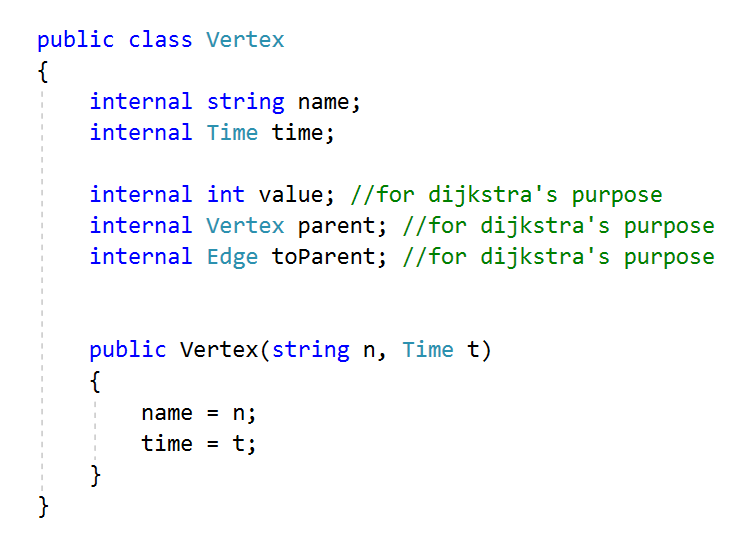
\includegraphics[width=0.7\linewidth]{./images/2_Vertex.png}}
  \caption{Rozšírená reprezentácia vrchola}
  \label{2_Vertex}
\end{figure}

Do objektu hrany sme zasiahli len minimálne: pridali sme jednu premennú hovoriacu či je daná hrana čakacia, čo nám pomôže pri výpise cesty, pretože z neho budeme chcieť takéto hrany vylúčiť.\newline

Táto reprezentácia údajov vyzerá naozaj sľubne, keďže algoritmus vyhľadávania na takto zostavenom grafe nebude potrebovať žiadne ďalšie úpravy.\newline


\section{Implementácia vyhľadávacieho algoritmu a výpis výsledku}

Nasledujúcim bodom bolo teda implementovať vyhľadávací algoritmus na pripravenej grafovej štruktúre. Ako sme už spomínali, na tento účel využijeme Dijkstrov algoritmus. Jeho implementácia podľa podkapitoly \ref{Dijkstra} je nenáročná. Za zmienku ale stojí pýtať sa, ktorý vrchol, po zadaní požiadavky používateľom, zvolíme ako počiatočný. Odpoveď je ale prostá: nájdeme vrchol s daným názvom, ktorý je čo najskôr po zadanom čase používateľa. Druhou možnosťou by bolo vytvoriť nový vrchol s parametrami od používateľa a ten umiestniť do grafu. Implementácia by bola jednoduchšia, ale oveľa viac mätúca. Rozhodli sme sa preto pre prvú možnosť.\newline

Opäť je vhodná chvíľa uvažovať. Ak bude náš graf rozsiahly, s čím musíme rátať, Dijkstrov algoritmus bude počítať veľmi dlho, než sa dopátra ku všetkým hodnotám. Rozumné je teda do implementácie zapojiť i ukončenie procesu vyhľadávania v nejakom rozumnom stave. Ako sme spomínali pri opisovaní Dijkstrovho algoritmu (\ref{Dijkstra}), mnoho implementácií končí po nájdený hodnoty najlacnejšej cesty pre zadaný konečný vrchol. My túto ideu v tejto chvíli aplikujeme, avšak jemne pozmenenú. Budeme si počas behu Dijkstrovho algoritmu počítať, koľko krát sme už prišli do finálneho vrchola a po určitom počte jeho návštev algoritmus ukončíme. Môžeme tak spraviť vďaka zmenenej štruktúre dát, keďže konečných vrcholov náš graf obsahuje viac, každý s inou hodnotou času. Otázkou zostáva, aký bude spomínaný počet návštev konečného vrchola. Ak bude priveľký, bude algoritmus bežať zbytočne dlho. Ak zasa malý, používateľ bude nespokojný pre nízky počet výsledkov. Navyše, v prípade opätovného vyhľadávania na tých istých vstupoch len s vyššou hodnotou tohto čísla bude musieť algoritmus začínať vždy odznova. Bolo by teda rozumné, nechať používateľov samých navoliť toto číslo. Nateraz sme ale túto hodnotu napevno zadrôtovali na číslo $3$. Naša implementácia algoritmu je k nahliadnutiu na obrázku \ref{Dijkstra_obr}. Treba podotknúť, že niektoré použité premenné sú definované mimo procedúry a ich význam je preto možne zistiť buď z názvu, z kontextu, alebo z prezretia si väčšej časti kódu.\newline

\begin{figure}[H]
  \centering{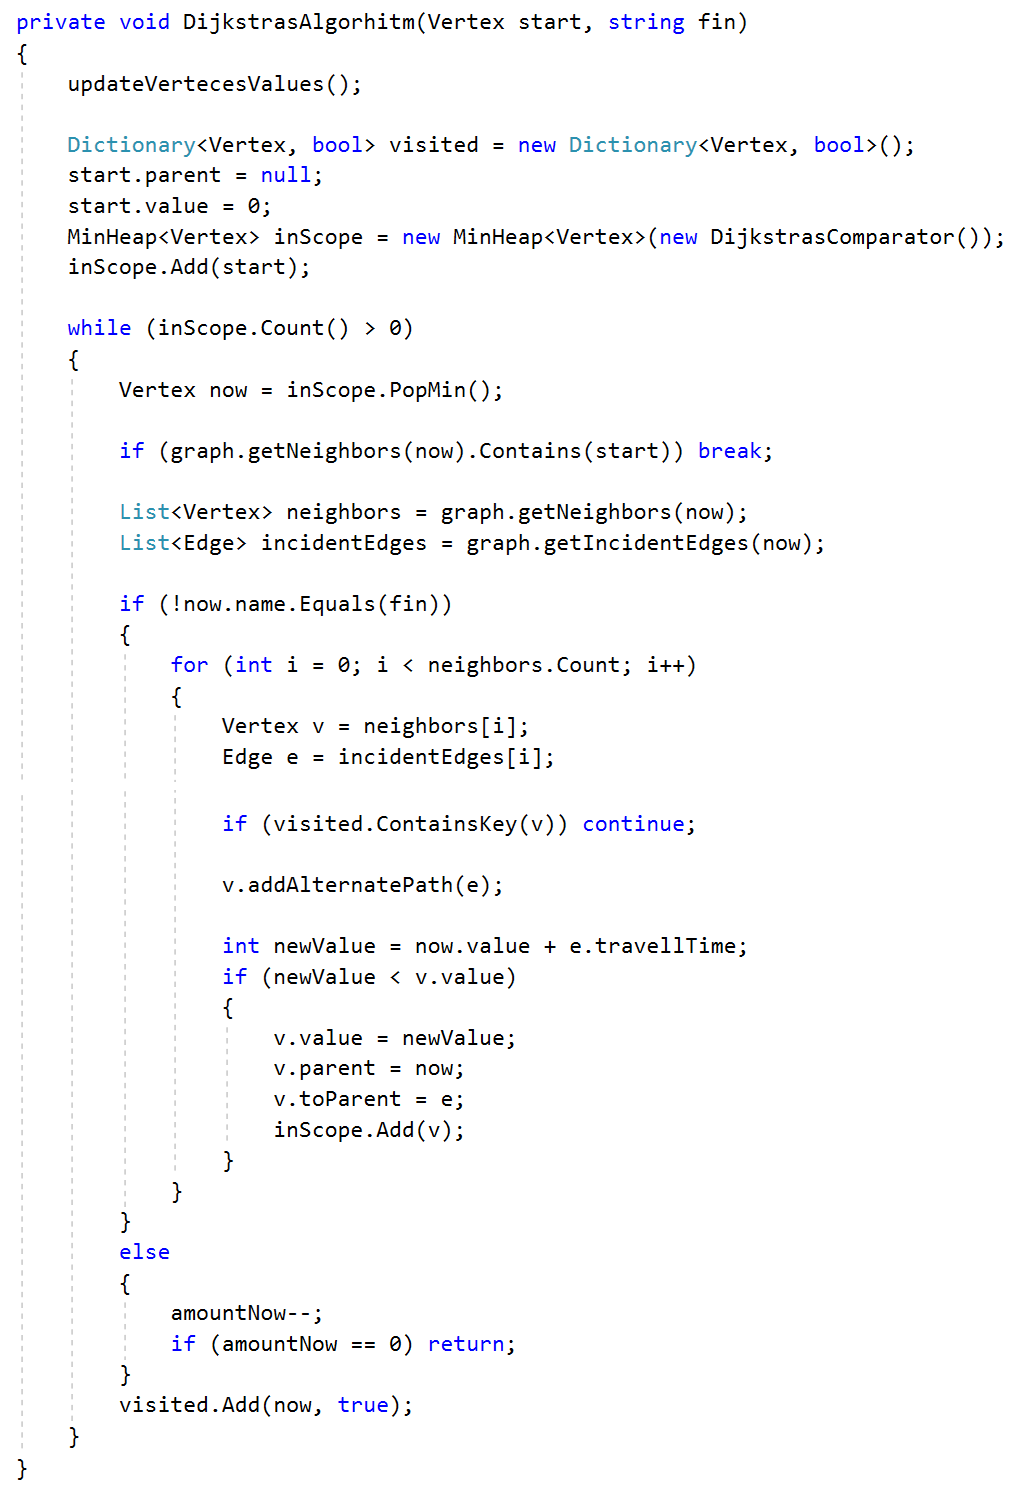
\includegraphics[width=0.7\linewidth]{./images/3_DijkstrovAlg.png}}
  \caption{Naša implementácia Dijkstrovho algoritmu}
  \label{Dijsktra_obr}
\end{figure}

Výsledná odpoveď algoritmu bude uložená vo vrcholoch grafu. Ich hodnoty pre požadovanú zastávku nájdeme jednoducho podľa názvu, teda vezmeme všetky vrcholy s názvom, aký je požadovaný a zoradíme ich podľa času počnúc zadaným časom pre vyhľadávanie. Pre nejaký rozumný počet týchto vrcholov necháme zrekonštruovať a do konzoly vypísať nájdené cesty. Táto hodnota by teda nemala a ani nemôže presiahnuť hodnotu návštev finálneho vrchola z predošlého odseku, momentálne teda $3$, nakoľko pre ostatné vrcholy už výslednú hodnotu nepoznáme.\newline

Vypisovanie cesty pre daný vrchol realizujeme pomocou rekurzie, čo nám zabezpečí správne poradie zastávok. Túto procedúru ukazuje obrázok \ref{PathShowing}. O samotný spôsob výpisu sa teda, ako je i zobrazené v kóde, stará iná trieda, trieda "PathShowing".\newline

\begin{figure}[H]
  \centering{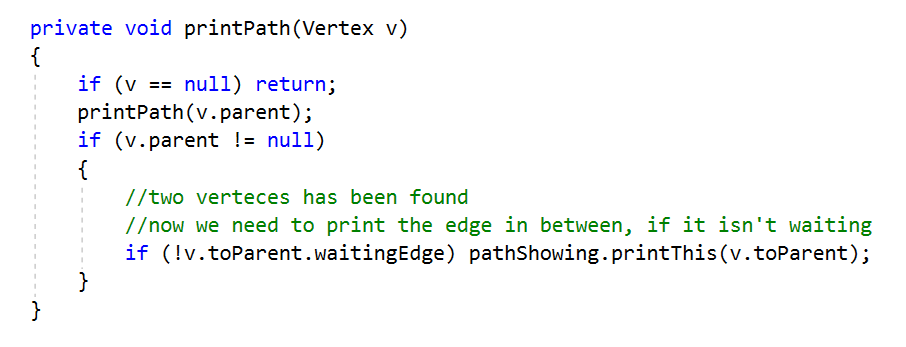
\includegraphics[width=\linewidth]{./images/3_PathShowing.png}}
  \caption{Kód starajúci sa o výpis cesty}
  \label{PathShowing}
\end{figure}


\section{Neefektívnosť vytvárania objektov}

Program, po implementácií všetkého doposiaľ opísaného, sa zdá byť funkčný. Na testovacích vstupoch je bezchybný. To však neznamená, že funkčný naozaj je. Aplikáciu musíme, čo je aj cieľom práce, otestovať na veľkých, respektíve reálnych dátach. Po spustení na týchto dátach už ale program nepracuje tak, ako by sme očakávali. Aplikácia sa i po viac ako hodinovom čakaní nerozbieha. Využili sme preto možnosť krokovania kódu, čím sme zistili príčinu nášho problému - aplikácií trvá pridlho pretváranie dát z obrovského textového súboru na žiadané objekty. Po prezretí si kódu sme, našťastie, našli neefektívne časti, ktoré sme prerobili. Presnejšie, pri vytváraní vrcholov sme zakaždým kontrolovali či už vrchol s rovnakými údajmi náhodou neexistuje, a tak aby sme nevytvorili vrcholy nesúce rovnaké informácie. Na to sme, pri našej jednoduchej implementácií grafu, museli prejsť poľom vrcholov. Preto sme do objektu grafu popridávali rôzne slovníky, resp. hashovacie mapy, čím sa nám podarilo výrazne urýchliť vytváranie objektov. Slovníky sme dokonca využili i počas algoritmu vyhľadávania, takže aj on sa stal trocha rýchlejším. Modifikovaná implementácia grafu sa nachádza na obrázku \ref{4_Graph}.\newline

\begin{figure}[H]
  \centering{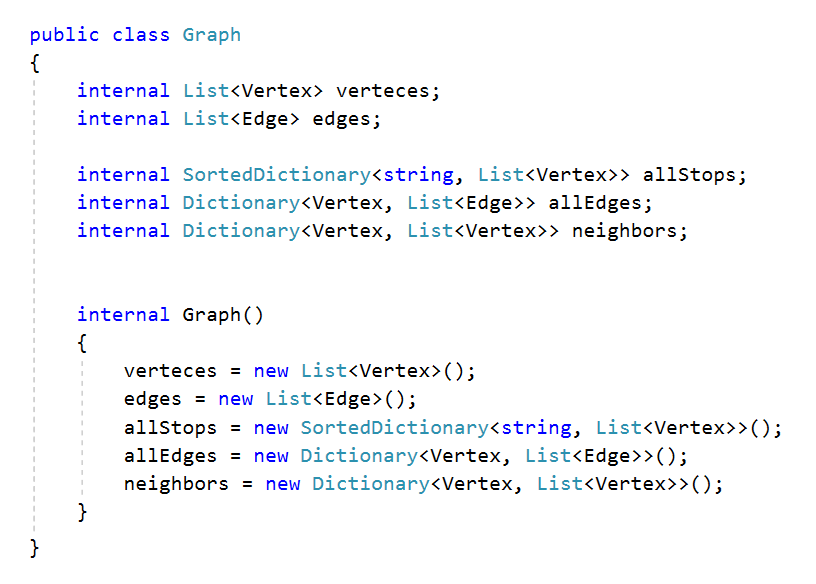
\includegraphics[width=\linewidth]{./images/4_Graph.png}}
  \caption{Vylepšená implementácia grafu}
  \label{4_Graph}
\end{figure}

Vylepšenie objektu grafu zabezpečilo, že sa aplikácia načítava približne minútu. Boli sme ju teda schopný otestovať na reálnych dátach a výsledky boli priaznivé. Dĺžka načítavania je ale stále neprajná, hoci aplikácia by mohla byť stále využiteľná, napríklad keby sa spustila a nechala bežať na serveri a používatelia by sa skrz určitú webovú stránku spytovali aplikácie svoje otázky.\newline


\section{Vyhľadávanie alternatívnych ciest}

Posledným cieľom našej práce je implementácia nejakého vylepšenia, ktoré obohatí náš program a urobí ho príťažlivejším. Rozhodli sme sa, že medzi funkcionalitu aplikácie pridáme možnosť zobrazenia alternatívnych ciest, keďže ju postráda skoro každý iný vyhľadávací nástroj. Presnejšie, pri zobrazení výsledkov algoritmu bude pri každej zastávke možné zvoliť zobrazenie iných trás do tej zastávky s príchodom v tom istom čase.\newline 

\begin{figure}[H]
  \centering{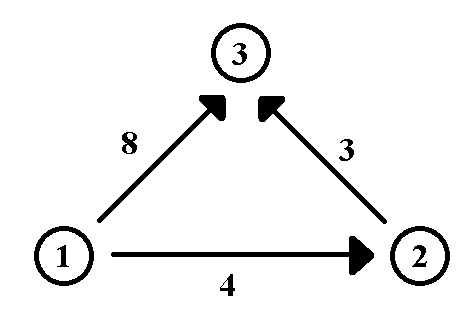
\includegraphics{./images/dijkstra_priklad.png}}
  \caption{Príklad alternatívnej trasy}
  \label{alternativ_priklad}
\end{figure}

Napríklad, pre graf zobrazený na \ref{alternativ_priklad} bude výsledok vyhľadávania cesta z vrcholu $1$ do $3$ cez vrchol $2$, nakoľko je najkratšia. Ale pri vrchole $3$ v zobrazení výsledku bude napísané, že doň vedú až dve cesty, nie len tá vypočítaná. Aplikácia bude schopná na žiadosť používateľa tieto alternatívne cesty vypísať a dokonca sa i navrátiť do predošlého stavu.\newline

Po dlhšom uvažovaní sme si uvedomili, že implementácia takéhoto vylepšenia nie je priveľmi náročná. Je ale nutné upraviť vyhľadávací algoritmus, čo ho, dúfame, príliš nezprehľadní. V prvom rade pridáme do triedy pre vrchol jedno pole hrán uchovávajúce si tie hrany, ktoré boli v Dijkstrovom algoritme skúšané ako kandidáti na najkratšiu cestu do tohto vrchola. Samozrejme, budú tam všetky - aj tie, ktorým sa nepodarilo, i tie, ktorým áno, lebo tie so zdarným porovnaním sa môžu neskôr prepísať inou, lepšou možnosťou. A ako sme už prezradili, úprava vo vyhľadávacom algoritme tiež nebude markantná. V ňom nám stačí pred porovnaním pridať hranu do spomínaného poľa pre cieľový vrchol daného vyhodnocovania.\newline

Idea je nasledovná: Uvažujme alternatívne cesty do vrchola $v$. Najskôr si musíme uvedomiť, ktoré to sú. Nech do vrchola $v$ smeruje $n$ hrán. Inak povedané, existuje $n$ hrán tvaru $xv$ pre ľubovoľný vrchol $x$. Potom vieme nájsť $n$ alternatívnych ciest do zvoleného vrchola, pre každú takúto hranu jednu, pričom každá cesta obsahuje ako poslednú hranu hranu $xv$ pre nejaký vrchol $x$ spojenú s najlacnejšou cestu do vrchola $x$ z počiatočného vrchola. Jej existenciu zaručuje Dijkstrov algoritmus, ktorý počíta všetky najlacejšie cesty z počiatočného vrcholu.\newline

Moze ich byt vela - vybrat par - utridit podla min ceny cesty co vrchola x.
zlozitost sa nezhorsi, iba ak pri utriedeni podla min..

Implementácia vylepšenia sa naozaj nezdá byť signifikantná, jej účel je ale naozaj prínosný. Avšak nie je pravda, že jej naprogramovanie je také jednoduché. S touto implementáciu sa nám podarilo získať výsledky, ktoré, žiaľ, nevieme vypísať. Vo výpise sa ale nachádza tvrdý oriešok. Keďže potrebujeme vypísať alternatívne cesty, potrebujeme nielen zmazať predošlý výpis výsledkov, ale si aj zapamätať tento stav, keďže sa k nemu bude chcieť používateľ pravdepodobne vrátiť. Ďalej, ak si zvolíme zobraziť alternatívne cesty pre nejakú zastávku, možno si budeme chcieť opäť z vypísaného zvoliť ďalšiu alternatívnu cestu. Výpis by teda mal fungovať do ľubovoľnej hĺbky. Ako nádherné riešenie tohto problému sa nám ponúka použiť návrhový vzor \textit{Memento}, ktorého \textit{Caretaker} si bude postupne zapamätávať stavy a na žiadosť nám posledný zapamätaný stav poskytne a zároveň ho odstráni zo svojej pamäte. Na jeho pamäť zasa poslúži dátová štruktúra \textit{zásobník} a ukladané stavy budú reprezentované triedou so zoznamom zoznamov hrán (zoznam hrán reprezentuje cestu a zoznam týchto ciest zas zobrazovaný výsledok). Implementácia \textit{Mementa} nám teda s prehľadom vyriešila všetky starosti.\newline

